\documentclass{revtex4-1}

\usepackage{amsmath}

\usepackage{bm}

\usepackage{physics}

\usepackage{algorithm}
\usepackage{algpseudocode}

\usepackage{graphicx}
\usepackage{subcaption}
\usepackage{epstopdf}
\graphicspath{{img/}}

\everymath{\displaystyle}

\begin{document}

\title{Restricted Boltzmann Machines}
\author{Giancarlo Fissore}
\date{May 2017}

\begin{abstract}
  Abstract text
\end{abstract}

\maketitle

\section{Introduction}

\section{Training Restricted Boltzmann Machines} \label{training}

\subsection{Definition of the model}

A Restricted Boltzmann Machine (RBM) is a model for neural networks which basically consists in a bipartite graph with a layer of hidden units \(h_i\) and a layer of visible units \(v_i\). The units in one layer are not connected among them but are connected to all the units in the other layer, as shown in fig. \ref{fig:rbm}. We restrict our treatment to the case of binary units \(h_i,v_i = 0,1\). Drawing a comparison between RBMs and spin models in statistical physics, we can define the following \textit{energy function}

\begin{equation}
E(\textbf{h},\textbf{v}) = - \sum_i a_i v_i - \sum_j b_j h_j - \sum_{i,j} v_i w_{ij} h_j
\label{eq:ef}
\end{equation}

where \(a_i\) and \(b_i\) are \textit{external fields} acting respectively on the visible and hidden units. The probability of a certain configuration is then given by the Boltzmann measure (taking \(\beta = 1\))

\begin{equation}
P(\textbf{h},\textbf{v}) = \frac{e^{-E(\textbf{h},\textbf{v})}}{Z}
\end{equation}

where \( \textstyle Z = \sum_{\textbf{h},\textbf{v}} e^{-E(\textbf{h},\textbf{v})}\) is the \textit{partition function}. The probabilities of activations for visible and hidden units can be simply computed to be

\begin{align}
P(v_i = 1 | \textbf{h}) &  = \frac{1}{1+e^{-a_i - \sum_{j} w_{ij} h_j}} \nonumber \\
& = sigm \left(a_i + \sum_{j} w_{ij} h_j \right)
\label{eq:act_vis}
\end{align}

\begin{align}
P(h_j = 1 | \textbf{v}) & = \frac{1}{1+e^{b_j + \sum_i w_{ij} v_i}} \nonumber \\
& = sigm \left(b_j + \sum_i w_{ij} v_i \right)
\label{eq:act_hid}
\end{align}

\begin{figure}
  \centering
  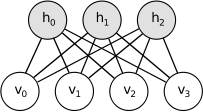
\includegraphics{rbm.png}
  \caption{bipartite structure of a RBM}
  \label{fig:rbm}
\end{figure}

We see that the usual neuron activation function (the sigmoid function, which we indicated by \(sigm\)) comes out naturally by choosing binary units. Moreover, we can now understand the importance of the external fields: they drive the activation of a certain unit by setting a threshold that has to be overcome by the opposite layer through the couplings \(w_{ij}\).

What we are interested in is the probability for the visible units, which is the layer we use to represent data. It can be easily defined as

\begin{align}
P(\textbf{v}) &  = \sum_{\textbf{h}} P(\textbf{h},\textbf{v}) \nonumber \\
& = \frac{e^{-F_c(\textbf{v})}}{Z}, \quad Z = \sum_{\textbf{v}} e^{-F_c(\textbf{v})}
\label{eq:p_model}
\end{align}

where, further exploiting the parallel with spin models, we have introduced the \textit{clamped free energy}

\begin{align}
F_c(\textbf{v}) & = -\log \sum_{\textbf{h}} e^{-E(\textbf{h},\textbf{v})} \nonumber \\
& = -\sum_i a_i v_i -\sum_j \log \left( 1 +  e^{\left( b_j + \sum_i w_{ij} v_i \right)} \right)
\end{align}

To use the RBM as a generative model, we want to maximize \(P(\textbf{v}\)) for the samples belonging to the training set. This is done by performing gradient ascent over the log-likelihood \(\log P(\textbf{v})\), whose derivative with respect to the weights can be computed to be

\begin{equation}
\frac{\partial \log P(\textbf{v})}{\partial w_{i,j}} = \langle h_i v_j \rangle_{data} - \langle h_i v_j \rangle_{model}
\label{eq:opt}
\end{equation}

where \(\langle \cdot \rangle_{data}\) denotes an average over the empirical distribution of the training set (\( \textstyle P_{data}(\mathbf{v}) = \frac{1}{N} \sum_{\mathbf{v}_n \in data} \delta (\mathbf{v} - \mathbf{v}_n ) \)) and 
\(\langle \cdot \rangle_{model}\) denotes the average over the distribution \eqref{eq:p_model}. Introducing the \textit{learning rate} \(\alpha \) (as a parameter for gradient ascent) we obtain an update rule for the weights matrix

\begin{equation}
\Delta \mathbf{W} = \alpha \left( \langle \mathbf{v h}^T \rangle_{data} - \langle \mathbf{v h}^T \rangle_{model} \right)
\label{eq:w_up}
\end{equation}

In the same way we can get the update rules for the external fields

\begin{align}
\Delta \mathbf{a} &= \alpha \left( \mathbf{v}_{data} - \mathbf{v}_{model} \right) \\
\Delta \mathbf{b} &= \alpha \left( \mathbf{h}_{data} - \mathbf{h}_{model} \right)
\end{align}

Given the update rules, the training consists in actually performing the gradient ascent. Once this is done, it is possible to sample the equilibrium configurations of the RBM to obtain samples which are generated according to the probability distribution of the training data. Unfortunately, the average over the model distribution \(\textstyle \langle \cdot \rangle_{model}\) is intractable as such term is exponential in the number of visible units. Approximations are then necessary to train and sample from a RBM; in particular Monte Carlo based algorithms are generally employed, such as \textit{k-steps contrastive divergence} (CDk) \cite{Hinton_CD}  and \textit{persistent contrastive divergence} (PCD) \cite{PCD}. Approximate algorithms based on mean-field methods from statistical physics have also been employed, but showing results of inferior quality with respect to CDk-PCD \cite{PCD}. Recently, however, a new algorithm based on mean-field has been proposed \cite{tap_train}, showing results comparable to the usual Monte Carlo based methods. An overview of this novel algorithm and an analysis of its performance is given in the next sections.

\subsection{Training via extended mean-field} \label{sec:emf}
We have already drawn attention to the similarities between the RBM model and spin models in statistical physics. In particular, the energy function \eqref{eq:ef} corresponds to the hamiltonian of the spin glass Sherrington-Kirkpatrick (SK) model \cite{SK} and this makes it possible to take advantage of well established results in spin glass theory to obtain a valid approximation to the intractable term in the update rule \eqref{eq:w_up}. In fact, looking back at the log-likelihood we can express it as

\begin{align}
\log P(\mathbf{v}) &= \log \frac{e^{-F_c(\mathbf{v})}}{Z} \\ \nonumber
&= -F_c(\mathbf{v}) - F
\end{align}

where \( \textstyle F = - \log Z \) is the \textit{free energy} of the SK model and it corresponds to the intractable term. Introducing the inverse temperature \(\beta\) we can write the Boltzmann measure of the SK model where the role of the spins is played by the units of the RBM and the separation between visible and hidden layers is retained only to make the connection between the two models clear

\begin{equation}
P(\textbf{h},\textbf{v}) = \frac{e^{- \beta E(\textbf{h},\textbf{v})}}{Z}
\end{equation}

By means of a high-temperature expansion (\(\beta \to 0\)) \cite{ht_exp} it is then possible to obtain the Thouless-Anderson-Palmer (TAP) expression for the free energy \cite{TAP} that, in the context of a RBM and truncated at second order, can be written as

\begin{align}
F_{TAP}(\mathbf{m}^v,\mathbf{m}^h) = &+ S(\mathbf{m}^v) + S(\mathbf{m}^h) \nonumber \\
&- \sum_i a_i m_i^v - \sum_j b_j m_j^h - \sum_{i,j} w_{i,j} m_i^v m_j^h \nonumber \\
&+ \sum_{i,j} \frac{w_{i,j}^2}{2} \left( m_i^v - {m_i^v}^2 \right) \left(m_j^v - {m_j^h}^2 \right) \label{eq:f_tap}
\end{align}

with \( \textstyle S(\mathbf{m}) = - \sum_i \left[ m_i \log m_i + (1 - m_i) \log (1 - m_i) \right] \).

We note that \(F_{TAP}\) is an \textit{effective free energy} expressed in terms of the magnetizations \(\mathbf{m}^v, \mathbf{m}^h\), given by eq. \eqref{eq:act_vis},\eqref{eq:act_hid}. Its minimization gives a valid approximation to the free energy \(F\)

\begin{equation}
F \simeq F_{TAP}(\mathbf{\tilde{m}}^v, \mathbf{\tilde{m}}^h), \qquad \left. \frac{dF_{TAP}}{d \mathbf{m}} \right\rvert_{\mathbf{\tilde{m}}^v, \mathbf{\tilde{m}}^h} = 0
\label{eq:f_approx}
\end{equation}

To obtain \(\mathbf{\tilde{m}}^v, \mathbf{\tilde{m}}^h\) it is then necessary to extremise \eqref{eq:f_tap} to obtain the following coupled equations

\begin{align}
m_i^v \simeq sigm \left\{ a_i + \sum_j \left[ w_{i,j} m_j^h - w_{i,j} \left( m_i^v - \frac{1}{2} \right) \left( m_j^h - {m_j^h}^2 \right) \right] \right\} \label{eq:tap_vis} \\
m_j^h \simeq sigm \left\{ b_j + \sum_i \left[ w_{i,j} m_i^v - w_{i,j} \left( m_j^h - \frac{1}{2} \right) \left( m_i^v - {m_i^v}^2 \right) \right] \right\} \label{eq:tap_hid}
\end{align}

that can be solved by iteration \cite{conv}. Finally, given the approximation to the free energy \eqref{eq:f_approx}, the optimization problem over the log-likelihood \eqref{eq:opt} is greatly simplified: the average over the training samples \(\textstyle \langle \cdot \rangle_{data}\) is unchanged while the intractable average over the model distribution \(\textstyle \langle \cdot \rangle_{model}\) is substituted by the maximization of \eqref{eq:f_approx}, giving

\begin{equation}
\Delta \mathbf{W} = \alpha \left( \langle \mathbf{v h}^T \rangle_{data} - \frac{\partial F_{TAP}(\mathbf{\tilde{m}}^v, \mathbf{\tilde{m}}^h)}{\partial w_{i,j}} \right)
\label{eq:w_up_tap}
\end{equation}

Summarizing, the training procedure based on TAP approximation is reported in the following algorithm.

\begin{algorithm}[H]
\caption{Extended mean-field training}\label{alg:tap}
\begin{algorithmic}[1]
\State \textbf{Data:} a training set of N data vectors
\State Randomly initialize the weights matrix \textbf{W}
\For{t = 0 to T (\# of epochs)}
  \ForAll{vectors in the training set}
    \State initialize  \(m_j^h=P(h_j|\mathbf{v}),m_i^v=P(v_i|\mathbf{h})\)
    \State iterate TAP equation \eqref{eq:tap_vis},\eqref{eq:tap_hid} to convergence to obtain \(\tilde{\mathbf{m}}^v,\tilde{\mathbf{m}}^h\)
    \State update \(\mathbf{W}\) with eq. \eqref{eq:w_up_tap}
  \EndFor
\EndFor
\end{algorithmic}
\end{algorithm}

We conclude by noting how the introduction of the inverse temperature \(\beta\) is just a formal passage; in the context of a RBM we keep \(\beta = 1\) and the high-temperature expansion is substituted by a weak-couplings expansion, under the assumption that the weights \(w_{ij}\) are small enough (this assumption is verified in next sections). The variance of the weights matrix can then serve as an \textit{effective inverse temperature}, giving

\begin{equation}
T_{eff} = \frac{1}{Var(\mathbf{W})}
\label{eq:t_eff}
\end{equation}

\subsection{Analysis of the learning}
To assess the performance of the extended mean-field (EMF) training described in section \ref{sec:emf} we have trained a RBM using both PCD and EMF and compared the outcomes, implementing both algorithms following the guidelines given in \cite{Hinton_guide}.

The dataset we used is the MNIST database \cite{mnist}, a set of \(70000\) handwritten digits whose samples consist in \(28 \times 28\) pixels centered and size-normalized images. The first \(60000\) samples are used for training the RBM while the remaining \(10000\) samples constitute the test set, that is used to validate the training and monitoring for overfitting. Examples of the MNIST samples are shown in fig. \ref{fig:samples_mnist}.

Drawing samples from the trained distribution \(P(\mathbf{v},\mathbf{h})\) is done by performing Gibbs sampling \cite{gibbs}, which basically consists in running a Markov chain to convergence. In the context of a RBM, as there are no links among units in the same layer, we can perform the sampling in blocks: starting from a visible configuration the conditional probability of the hidden layer is computed using \eqref{eq:act_hid} and this makes it possible to compute the conditional probability of the visible layer, starting a loop that if iterated long enough is guaranteed to produce samples approximating the joint probability distribution of all the variables. The sampling algorithm is reported below for clarity.

\begin{algorithm}[H]
\caption{Gibbs sampling}\label{alg:gibbs}
\begin{algorithmic}[1]
\State \textbf{Init:} take a random sample \(\mathbf{v}\)
\For{i=0 to k}
  \State \( \mathbf{h} = P(\mathbf{h}|\mathbf{v}) \)
  \State \( \mathbf{v} = P(\mathbf{v}|\mathbf{h}) \)
\EndFor
\State Set \(v_i = 1\) with probability \(P(v_i = 1|\mathbf{h})\)
\end{algorithmic}
\end{algorithm}

The results of the training are affected by many parameters, that we have set empirically and in accordance to \cite{PCD}\cite{tap_train}. A summary for our choices is given below:

\begin{itemize}
  \item \(\sigma_v = 0.01\): this is the variance for the initialization of the weights \(\mathbf{W}\) as a gaussian random matrix. This value is agreed to work well and it fits our requirement of having small weights in order to perform the weak couplings expansion
  \item \(\alpha = 0.01\): a larger learning rate would speed up the training but making the RBM initially learn a bad model of the data that is then difficult to refine during succeeding epochs. A small learning rate is then preferred to obtain a good generative model.
  \item \(d = 784\): number of visible units, set in accordance to the dimensionality of MNIST images (\(28 \times 28\)).
  \item \(p = 500\): number of hidden units, set in accordance to other works on the MNIST database. A too small number would not make it possible to accurately represent all the characteristics of the training data while a too big number would result in a redundant increase in the complexity of the model.
  \item batch size \(m = 100\): training data are not processed one by one but in batches, so that the operations can be vectorized to speed up the learning. The higher the batch size, the more efficient the learning. Lower batch sizes, however, are found to give better generative models and in our case the chosen value is a good trade-off.
  \item \( k = 15 \): number of Gibbs sampling steps used for PCD learning. For EMF, we recall that no Gibbs sampling steps are necessary during training.
\end{itemize}

\begin{figure}
  \centering
  \begin{subfigure}{.25\linewidth}
    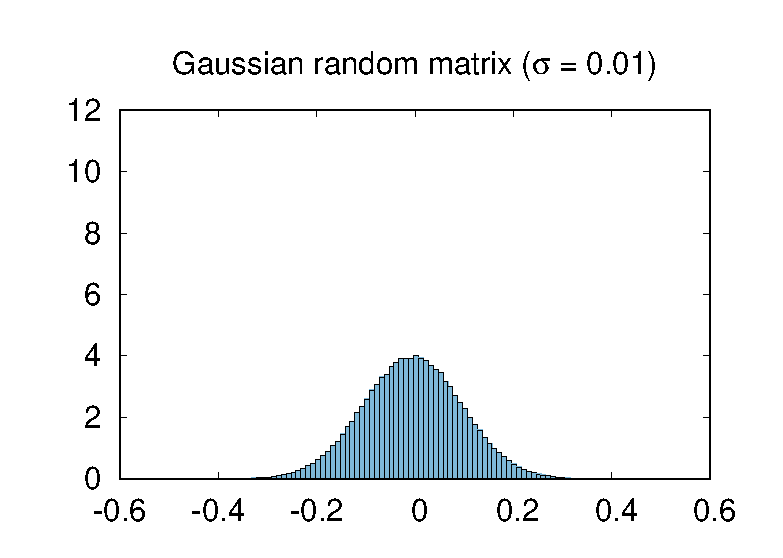
\includegraphics[width=\linewidth]{w_init.eps}
    \caption{}
    \label{fig:w_init}
  \end{subfigure}
  \begin{subfigure}{.25\linewidth}
    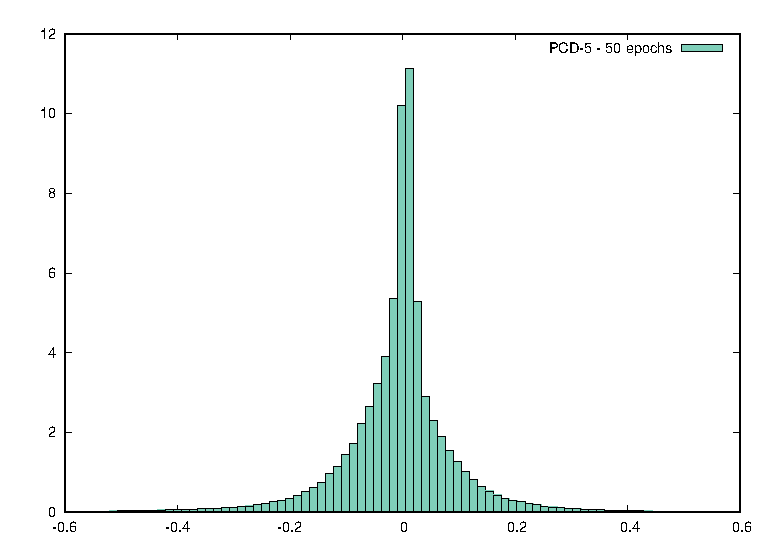
\includegraphics[width=\linewidth]{w_pcd5_50.eps}
    \caption{}
    \label{fig:w_pcd5_50}
  \end{subfigure}
  \begin{subfigure}{.25\linewidth}
    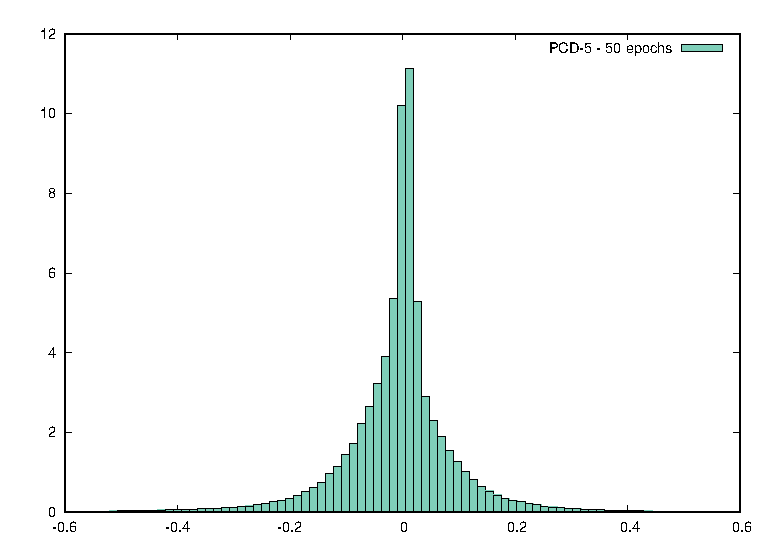
\includegraphics[width=\linewidth]{w_pcd5_50.eps}
    \caption{}
    \label{fig:w_tap20_50}
  \end{subfigure}\par\medskip
  \begin{subfigure}{.25\linewidth}
    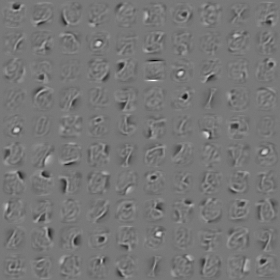
\includegraphics[width=\linewidth]{features_pcd.png}
    \caption{}
    \label{fig:features_pcd}
  \end{subfigure}
  \begin{subfigure}{.25\linewidth}
    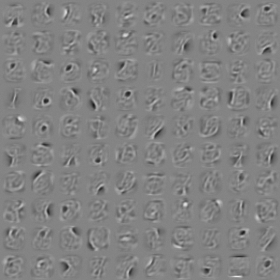
\includegraphics[width=\linewidth]{features_tap.png}
    \caption{} 
    \label{fig:features_tap}
  \end{subfigure}
  \begin{subfigure}{.25\linewidth}
  	\begin{subfigure}{\linewidth}
  		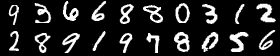
\includegraphics[width=\linewidth]{samples.png}
        \caption{} 
        \label{fig:samples_mnist}
  	\end{subfigure}
  	\begin{subfigure}{\linewidth}
  		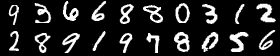
\includegraphics[width=\linewidth]{samples.png}
        \caption{} 
        \label{fig:samples_pcd}
  	\end{subfigure}
  	\begin{subfigure}{\linewidth}
  		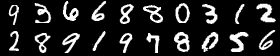
\includegraphics[width=\linewidth]{samples.png}
        \caption{} 
        \label{fig:samples_tap}
  	\end{subfigure}
  \end{subfigure}
  
 \caption{}
\end{figure}

The comparison between PCD and EMF is performed by looking at the weights distribution, the generated hidden features and the samples generated by the trained RBM.

The weights distribution after training is shown in fig. \ref{fig:w_pcd5_50}-\ref{fig:w_tap20_50}. For both PCD and EMF the initial gaussian distribution is shrinked to a more peaked distribution around zero, showing the equivalence of the two methods from this point of view. In the EMF framework this legitimates the weak-couplings expansion and shows how the learning procedure determines an increase in the effective temperature \eqref{eq:t_eff}. In fig. \ref{fig:features_pcd}-\ref{fig:features_tap}, instead, the hidden features generated by the RBM are shown. Each consists in the activation pattern of the visible layer driven by a single hidden unit, whose ensemble corresponds to the strokes by which the samples generated by the RBM are composed. [comment].

The most significant comparison between the two methods is given by looking at the samples generated by the trained models, shown in fig. \ref{fig:samples_pcd}-\ref{fig:samples_tap}. Both methods generate good models of the training data, but we can see that for EMF some samples are not resembling real digits. This is not surprising if we take into account the fact that the TAP free energy \eqref{eq:f_tap} employed in EMF encodes also the metastable states of the corresponding physical system.

As a conclusion, we see that PCD and EMF training give comparable results, apart from the spurious states generated by EMF. The strength of EMF, however, is the ability to provide a theoretical framework that can be helpful in trying to understand what is going on during the learning. A careful analysis of the RBM from the point of view of statistical physics should be able to provide useful insights on its functioning and provide a solution to the problems of EMF. Some work has been done in this direction.

% A quantitative criterium of caomparison is given by looking at the pseudo-likelihood for PCD \cite{Hinton_guide} and the EMF-likelihood for EMF \cite{tap_train}, fig. \ref{fig:likelihood}. The two objective functions are different and a direct caomparison of their values is not clearly meaningful, even if the similarity is striking. 

\section{Singular Values Decomposition of a RBM}
The structure of the samples that a RBM  is able to generate must be in some way encoded into the external fields \(\mathbf{a},\mathbf{b}\) and the weights matrix \(\mathbf{W}\), as these are the set of quantities which constitute the RBM itself. For what concerns the visible field values \(a_i\), these are used to make sure that the visible unit \(i\) is activated with a probability \(p_i\) given by the proportion of training samples in which unit \(i\) is active (i.e. where its value is 1). No learning is needed to make the field \(\mathbf{a}\) encode this information, it is sufficient to use the initialization rule

\begin{equation}
a_i = \log[p_i/(1-p_i)]
\label{eq:bias_init}
\end{equation}

as reported in \cite{Hinton_guide}. To understand how the structure of the data is encoded into the weights matrix, instead, we monitored the singular value decomposition (SVD) of \(\mathbf{W}\) during the training.

\subsection{Informal introduction to Singular Value Decomposition (SVD) and Principal Component Analysis (PCA)}

The Principal Component Analysis (PCA) technique can be introduced by considering the covariance matrix of a dataset. Given a data matrix \(\mathbf{X}\) of dimension \(n \times p\) with \(n > p\), where \(n\) is the number of samples and \(p\) is the dimension of each sample, and further assuming that samples are centered (i.e. column means have been subtracted, as data are arranged by rows), we can define an unbiased estimator for the related covariance matrice (square and symmetric)

 %Given a \(n \times p\) data matrix \(\mathbf{X}\) where the samples are arranged by rows and centered (i.e. column means have been subtracted), we can define an unbiased estimator for the related covariance matrice (square and symmetric)

\begin{equation}
\mathbf{C} = \frac{\mathbf{X}^T \mathbf{X}}{n-1}
\end{equation}

that can be diagonalized

\begin{equation}
\mathbf{C} = \mathbf{V L V}^T
\end{equation}

where the columns of \(\mathbf{V}\) are eigenvectors of \(\mathbf{C}\) and \(\mathbf{L}\) is the diagonal matrix of the eigenvalues \(\lambda_i\). Projecting the samples over the eigenvectors of the covariance matrix (also called \textit{principal directions} in the context of PCA) we obtain the \textit{principal components}: new, independent variables that account for the maximum possible variability in the data. More precisely, the first \textit{principal component} maximizes the variance of the projections of the data (i.e. it has the highest possible variance) and the succeeding components maximize the variance while satisfying the constraints of being orthogonal to the preceeding components. A rigorous demonstration of the properties of \textit{principal components} is given in [].

The Singular Value Decomposition (SVD) is the generalization of eigenmodes decomposition to rectangular matrices, and it is given by

\begin{equation}
\mathbf{X} = \mathbf{U \Sigma} \mathbf{V}^T
\end{equation}

where \(\mathbf{U}\) is an orthogonal \(n \times p\)  matrix whose columns are the \textit{left singular vectors} \(\mathbf{\mu}_j \), \(\mathbf{V}\) is an orthogonal \(p \times p\) matrix whose columns are the \textit{right singular vectors} \( \mathbf{\nu}_j \) and \( \mathbf{\Sigma} \) is a diagonal \(p \times p\) matrix whose elements are the singular values \(\sigma_j\). The separation into left and right singular vectors is due to the rectangular nature of the decomposed matrix, and the similarity with eigenmodes decomposition is revealed by the following SVD equations

\begin{align}
\mathbf{X} \mathbf{\nu}_j & = \sigma_j \mathbf{\mu}_j \\
\mathbf{X}^T \mathbf{\mu}_j & = \sigma_j \mathbf{\nu}_j
\end{align}

Plugging the SVD of \(\mathbf{X}\) into the definition of covariance matrix

\begin{align}
\mathbf{C} & = \frac{\mathbf{X}^T \mathbf{X}}{n-1} = \frac{\mathbf{V \Sigma U}^T \mathbf{U \Sigma V}^T}{n-1}  \\ \nonumber
& = \mathbf{V} \frac{\mathbf{\Sigma}^2}{n-1} \mathbf{V}^T \nonumber 
\end{align}

we see how the \textit{right singular vectors} can be identified as the \textit{principal directions} and a relation between the singular values \(\sigma_j\) and the eigenvalues of the covariance matrice \(\lambda_j\) is easily found

\begin{equation}
\lambda_j = \frac{\sigma_j}{n-1}
\label{eq:ls_map}
\end{equation}

Finally, the \textit{principal components} are given by \(\mathbf{U \Sigma}\) (\(\mathbf{XV} = \mathbf{U \Sigma V}^T \mathbf{V} = \mathbf{U \Sigma}\)).

In the context of a RBM, we are interested in analyzing the SVD of the weights matrix \(\mathbf{W}\)

\begin{equation}
\mathbf{W} = \mathbf{U \Sigma V}^T
\end{equation}

Motivation for this analysis is suggested by looking at the linearized mean-field equations of our model. As there are not connections among variables in the same layer, the magnetizations \(m_i^v,m_j^h\) are given by eq. \eqref{eq:act_vis},\eqref{eq:act_hid} and the mean-field equations are

\begin{equation}
m_i^v = sigm \left(a_i + \sum_{j} w_{ij} m_j^h \right)
\end{equation}

\begin{equation}
m_j^h = sigm \left(b_j + \sum_i w_{ij} m^v_i \right)
\end{equation}

In section \ref{training} we have seen that the weights \(w_{i,j}\) are small (both at the beginning and after the training) and how we can get rid of the external visible field by centering the training data. The external hidden field is instead initialized to zero and it varies slowly, so it doesn't have any effects at the beginning of the training. Thus, neglecting both the external fields we can linearize the mean-field equations to obtain (defining \( \tilde{m}_i^v = m_i^v - 1/2, \tilde{m}_j^h = m_j^h - 1/2 \) for convenience)

\begin{equation}
\tilde{m}_i^v \simeq \frac{1}{4} \sum_j w_{i,j} \tilde{m}_j^h
\label{eq:mf_vis}
\end{equation}

\begin{equation}
\tilde{m}_j^h \simeq \frac{1}{4} \sum_i w_{i,j} \tilde{m}_i^v
\end{equation}

We can now express the weights \(w_{i,j}\) in terms of the SVD as (\(u_{i,\alpha}\) identifies the \(i_{th}\) component of the \(\alpha_{th}\) columns of \(\mathbf{U}\), and analogous notation is used for \(\mathbf{V}\))

\begin{equation}
w_{i,j} = \sum_{\alpha} \sigma_{\alpha} u_{i,\alpha} v_{j,\alpha}
\label{eq:w_exp}
\end{equation}

and expand the magnetizations over the singular vectors

\begin{equation}
\tilde{m}_{\alpha}^v = \sum_i u_{i,\alpha} \tilde{m}_i^v
\label{eq:mv_exp}
\end{equation}

\begin{equation}
\tilde{m}_{\alpha}^h = \sum_j v_{j,\alpha} \tilde{m}_j^h
\end{equation}

Combining eq. \eqref{eq:mf_vis},\eqref{eq:w_exp},\eqref{eq:mv_exp} and recalling that the columns of \(\mathbf{U}\) form an orthonormal basis, we get

\begin{align*}
\tilde{m}_{\alpha}^v & = \frac{1}{4} \sum_{\alpha '} \sigma_{\alpha} \delta_{\alpha,\alpha '} \tilde{m}_{\alpha}^h \\ \nonumber
& = \frac{1}{4} \sigma_{\alpha} \tilde{m}_{\alpha}^h \nonumber
\end{align*}

We can proceed in an analogous way with \(\tilde{m}_{\alpha}^h\) to finally obtain the coupled linear equations

\begin{equation}
\tilde{m}_{\alpha}^v = \frac{1}{4} \sigma_{\alpha} \tilde{m}_{\alpha}^h
\end{equation}

\begin{equation}
\tilde{m}_{\alpha}^h = \frac{1}{4} \sigma_{\alpha} \tilde{m}_{\alpha}^v
\end{equation}

These equations show how the magnetizations aligned to the singular vectors with a strong \(\sigma_{\alpha}\) are amplified, while magnetizations related to small \(\sigma_{\alpha}\) are penalized. We then expect the samples generated by a trained RBM to be affine to the strongest singular vectors, and we can try to understand how. To this end, we can better specify the role of the SVD matrices in the context of a RBM:

\begin{itemize}
\item \(\mathbf{U}\) encodes the singular vectors related to the visible layer; these can be visualized in the pixel space and basically consist in the principal components of \(\mathbf{W}\).
\item  \(\mathbf{V}\) is related to the hidden layer; it is a square orthogonal matrix that can be interpreted as a rotation and its columns are the principal directions of \(\mathbf{W}\).
\item The singular values \( {\sigma}_j \) contained in \(\mathbf{\Sigma}\) can be thought of as scaling factors whose action is to weight the singular vectors composing \(\mathbf{W}\).
\end{itemize}

Given the above characteristics we focused our attention on \(\mathbf{\Sigma}\) and \(\mathbf{U}\), tracking the distribution of the singular values and looking at the corresponding left singular vectors during the training.

\subsection{Distribution of the singular values}
The weights matrix W is initialized as a gaussian random matrix with variance \(\sigma_v\) (and zero mean). The eigenvalues distribution of the corresponding symmetric square matrix \(\mathbf{W}^T \mathbf{W} \) is known to be given by the Marchenko-Pastur law \cite{MP_law} in its canonical form. The singular values \(\sigma_j\) are related to the eigenvalues \(\lambda_j\) by \eqref{eq:ls_map}, and by defining the parameter \( r = p/d \), with \(p\) the size of the hidden layer and \(d\) the size of the visible layer (we recall that \(\mathbf{W}\) is a \(d \times p\) matrix), the expression of the Marchenko-Pastur law is given by (in the limit \( p,d \to \infty \) with \(r\) finite)

\begin{equation}
\rho (\lambda) = \frac{1}{2 \pi \sigma_v^2} \frac{\sqrt{(\lambda - r_-)(r_+ - \lambda)}}{r \lambda}
\end{equation}

where the higher and lower bounds \(r_{\pm}\) are

\begin{equation}
r_{\pm} = \sigma_v^2 \left(1 \pm \sqrt{r} \right)^2
\end{equation}

Fig. \ref{fig:mp_fit} shows the agreement between the empirical distribution and the theoretical distribution. In particular, we note how all \(\sigma_j\) have values below the threshold set by the Marchenko-Pastur law, forming a \textit{bulk} of singular values.

\begin{figure}
  \centering
  \begin{subfigure}{.25\linewidth}
    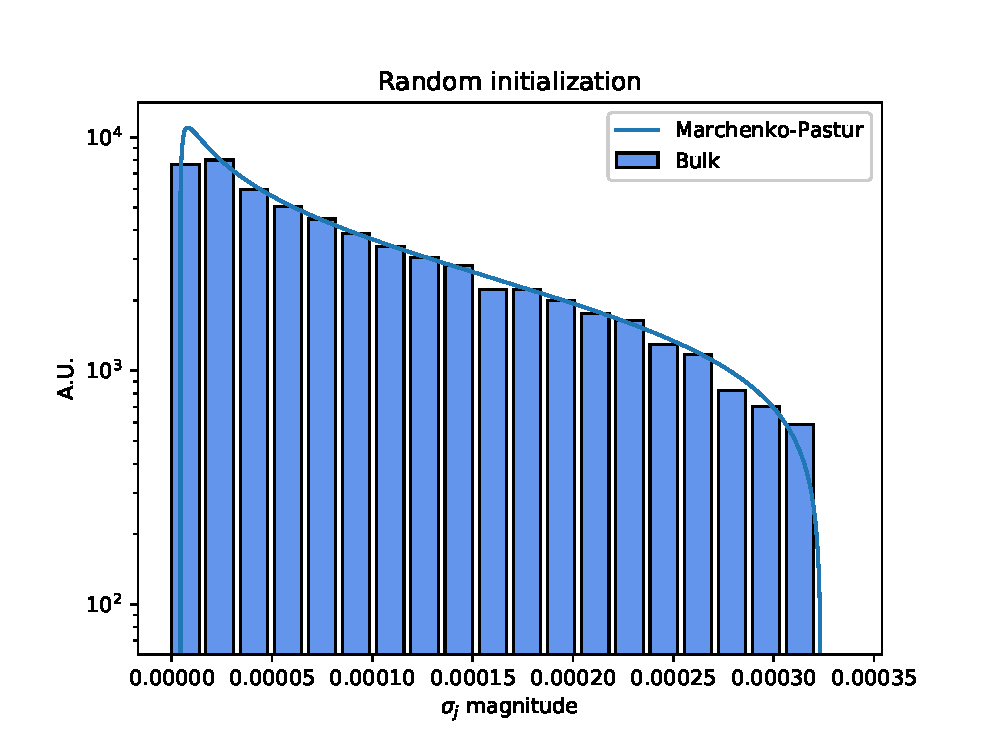
\includegraphics[width=\linewidth]{mp_fit.eps}
    \caption{}
    \label{fig:mp_fit}
  \end{subfigure}
  \begin{subfigure}{.25\linewidth}
    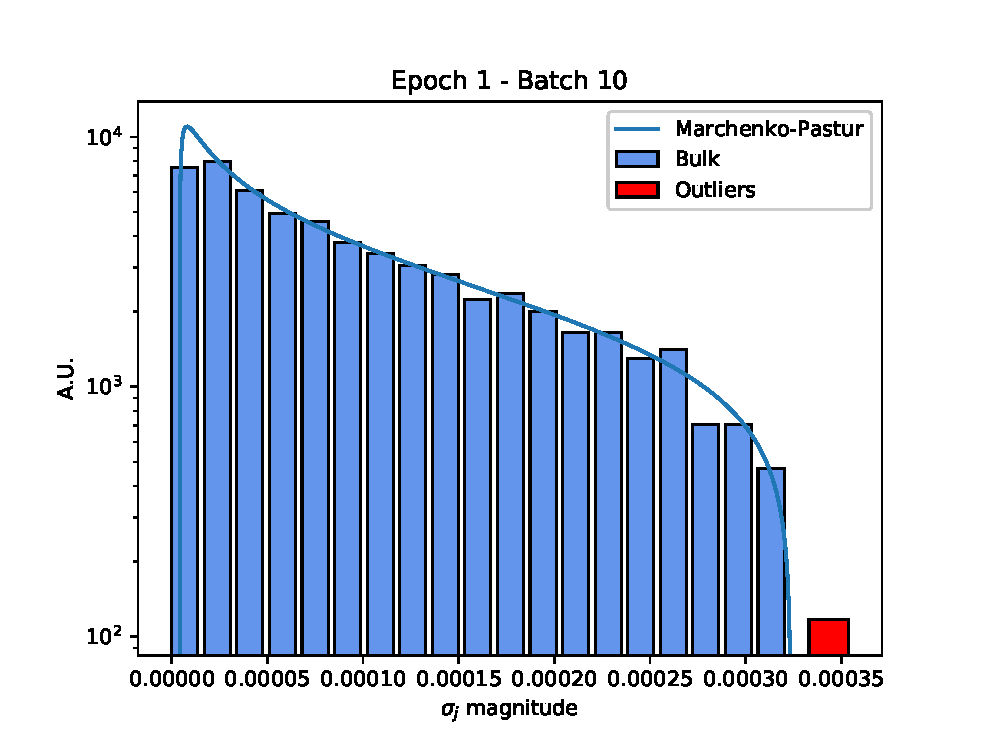
\includegraphics[width=\linewidth]{sv_distr_e1_b10.eps}
    \caption{}
    \label{fig:sv1}
  \end{subfigure}\par\medskip
  \begin{subfigure}{.25\linewidth}
    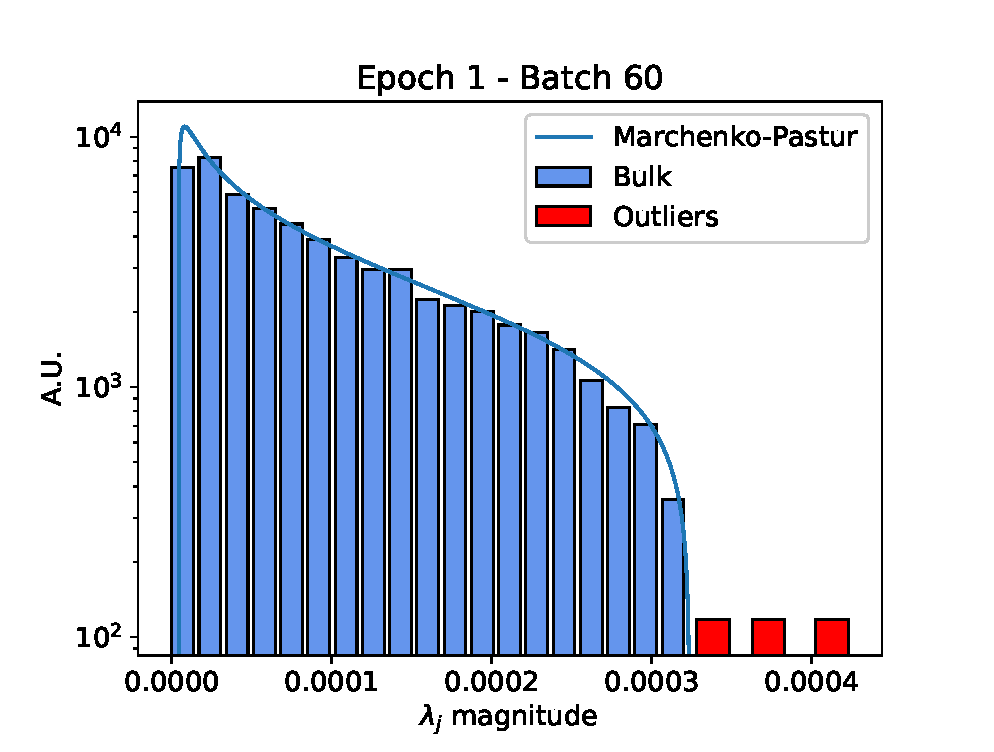
\includegraphics[width=\linewidth]{sv_distr_e1_b60.eps}
    \caption{}
    \label{fig:sv2}
  \end{subfigure}
  \begin{subfigure}{.25\linewidth}
    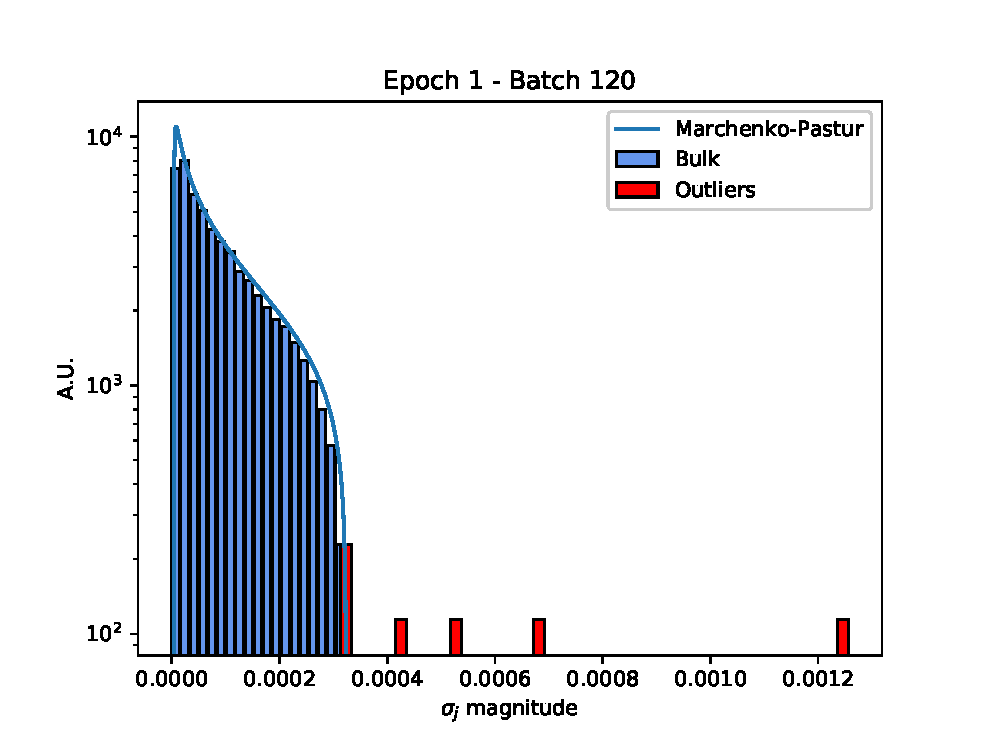
\includegraphics[width=\linewidth]{sv_distr_e1_b120.eps}
    \caption{} 
    \label{fig:sv3}
  \end{subfigure}
  \begin{subfigure}{.5\linewidth}
    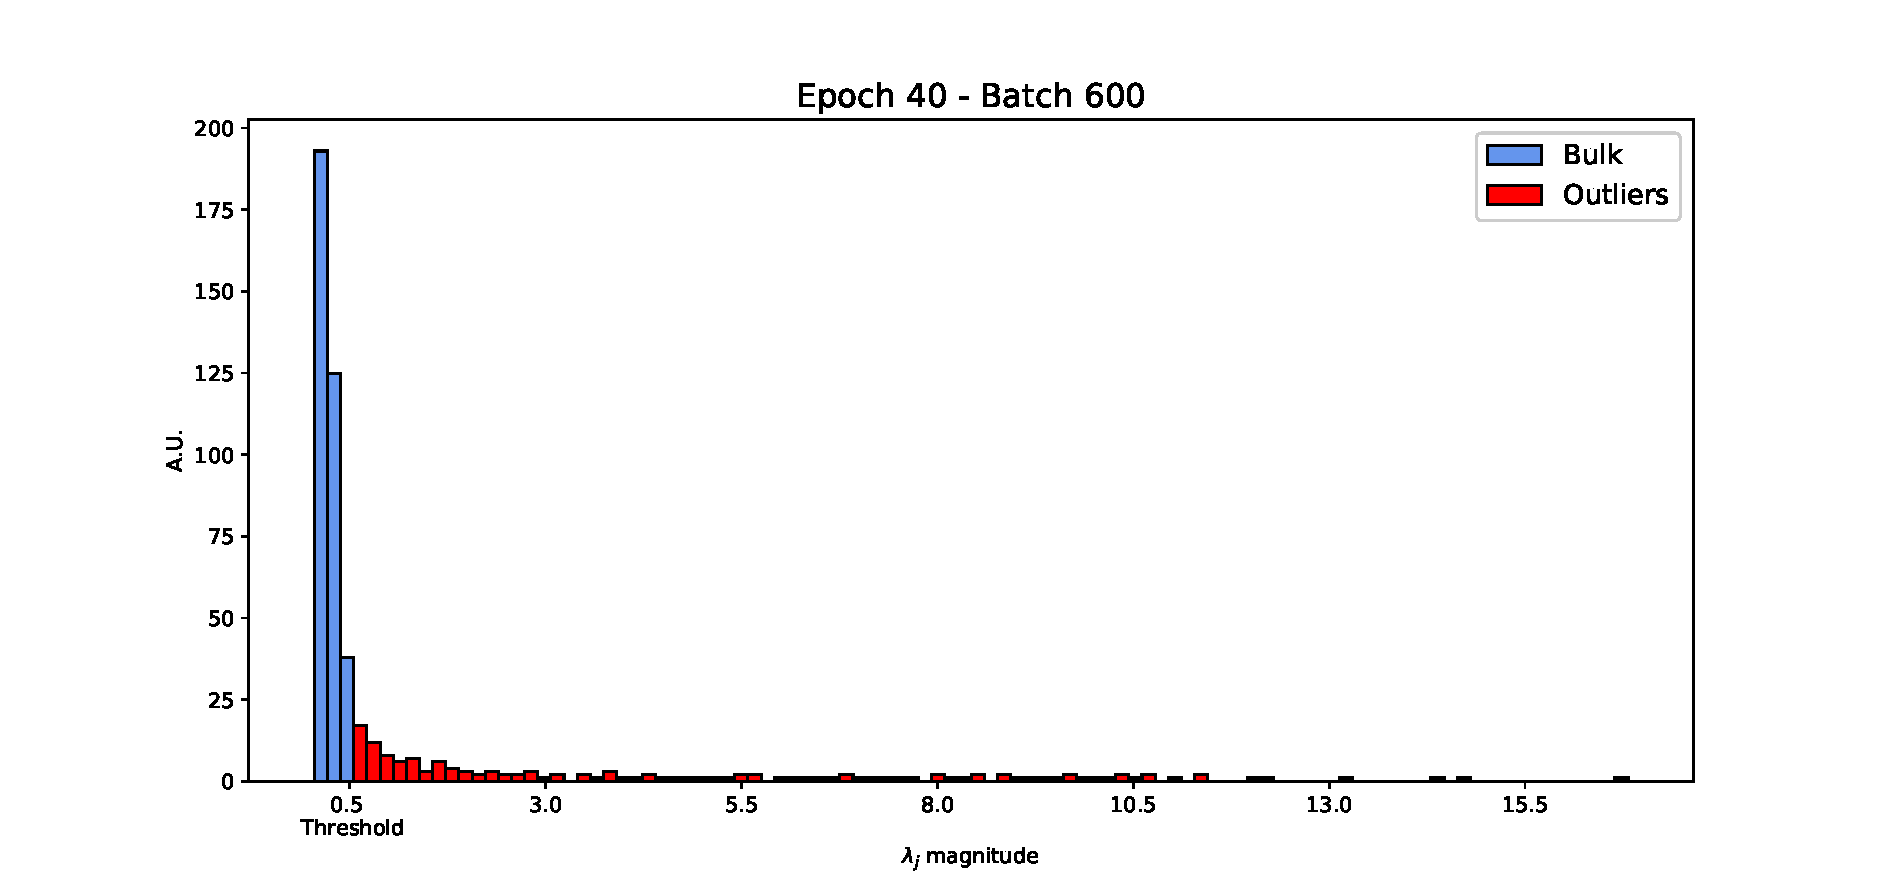
\includegraphics[width=\linewidth]{sv_distr_e40_b600.eps}
    \caption{}  
    \label{fig:sv4}
  \end{subfigure}
 \caption{\textbf{(a)} Singular values distribution of the initial random matrix compared to Marchenko-Pastur law. \textbf{(b)-(d)} With the training we can see some singular values strengthening and overcoming the threshold set by the Marchenko-Pastur law. \textbf{(e)} Distribution of the singular values after a long training: we can see many outliers spread above threshold and a spike of below-threshold singular values near zero}
\end{figure}

Starting with the training we see that many singular values increase in magnitude and overcome the threshold for a gaussian random matrix; these are \textit{outliers} leaving the bulk, shown in fig. \ref{fig:sv1}-\ref{fig:sv3}. During the first epochs of the training this process is very fast and many \(\sigma_j\) are easily extracted from the bulk, growing of many orders of magnitude. The bulk is instead shrinked to low values, meaning that the \(\sigma_j\) that do not overcome the threshold decrease in magnitude. Going on with the training this process slows down but it does not stop: outliers keep growing slowly and the bulk keeps shrinking to approach a spike around zero. It is important to note that a kind of hierarchy is maintained in the process: the first outliers are never overcome by the newly extracted \(\sigma_j\), and this is made clear by looking at the corresponding left singular vectors (see next section).
After a long training the singular values \(\sigma_j\) are separated into two categories: a concentrated set of almost-null singular values and a set of outliers spread above the threshold, as shown in fig. \ref{fig:sv4}.

The evolution of the \(\sigma_j\) distribution described above suggests that the training process is able to discern between the \textit{most important} singular vectors, that are brought above threshold first and heavily strengthen, and a bulk of \textit{less important} singular vectors, that end up above threshold but whose \( \sigma_j\) reach values order of magnitude smaller then those of the strongest singular vectors. Moreover, the below-threshold singular vectors are practically eliminated by cutting down the corresponding \(\sigma_j\).

These observations give a good indication about what are the dynamics of the learning process, but there are some matters that need to be addressed: (i) it is not clear what singular vectors actually represent, (ii) the meaning of \textit{more} and \textit{less} important singular vectors has to be specified, (iii) no clues about stopping criteria for the learning are given.

\subsection{Analysis of left singular vectors}

To understand the role of the left singular vectors of a RBM we must keep in mind the interpretation for the SVD decomposition of \textbf{W} given previously. We have seen how the matrix of the weights \textbf{\(\Sigma\)} is shaped during the learning, and we recall that \textbf{V} is interpreted as a rotation in the space of the hidden units. We then expect to recover the structure of the training data into the \textbf{U} matrix, and to show this we carefully analyze the left singular vectors during training by visualizing them in the pixel space.

Before focusing on the left singular vectors, we note that also the external visible field can be visualized in the pixel space. With the initialization rule \eqref{eq:bias_init} we are able to encode into the field the mean activation of the visible layer, which is clearly shown in fig. \ref{fig:vbias} in the pixel space. If we instead initialize the visible field with a null vector, the mean activation pattern is learnt very effectively as the strongest left singular vector. The striking resemblance between the mean activation pattern computed from the training data and the one learnt by the RBM is shown in fig. \ref{fig:m1tr}-\ref{fig:vbias} and it serves as a first example of what the left singular vectors represent. It seems then equivalent to either encode the mean activation pattern into the visible field since the beginning or letting the RBM learn such a pattern as a left singular vector. In practice the second case is not desirable as the RBM associates to the mean activation pattern a very strong singular value, many order of magnitudes higher then the strongest outliers. This results in a bias in the sampling from the trained machine, such that the samples whose activation pattern is nearest to the mean are sampled with a higher frequency (in the worst case those are the only configurations sampled at equilibrium).

\begin{figure}
  \centering
  \begin{subfigure}{.15\linewidth}
    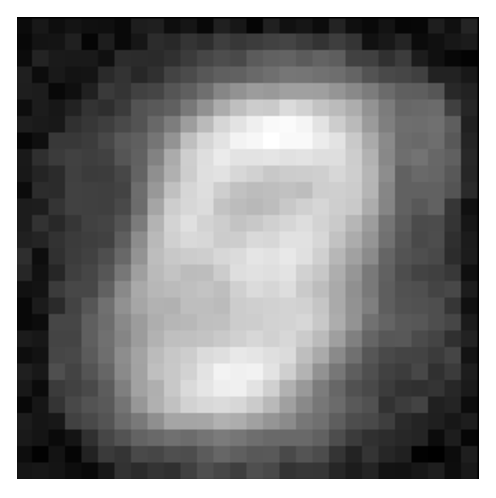
\includegraphics[width=\linewidth]{mode_1_training.eps}
    \caption{}
    \label{fig:m1tr}
  \end{subfigure}
  \begin{subfigure}{.15\linewidth}
    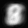
\includegraphics[width=\linewidth]{vbias.png}
    \caption{}
    \label{fig:vbias}
  \end{subfigure}
  \begin{subfigure}{.15\linewidth}
    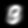
\includegraphics[width=\linewidth]{X_l_eigv_1.png}
    \caption{}
    \label{fig:m1data}
  \end{subfigure}\par\medskip
  \begin{subfigure}{\linewidth}
    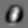
\includegraphics[width=.05\linewidth]{X_l_eigv_2.png}
    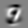
\includegraphics[width=.05\linewidth]{X_l_eigv_3.png}
    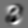
\includegraphics[width=.05\linewidth]{X_l_eigv_4.png}
    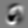
\includegraphics[width=.05\linewidth]{X_l_eigv_5.png}
    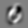
\includegraphics[width=.05\linewidth]{X_l_eigv_6.png}
    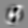
\includegraphics[width=.05\linewidth]{X_l_eigv_7.png}
    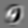
\includegraphics[width=.05\linewidth]{X_l_eigv_8.png}
    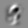
\includegraphics[width=.05\linewidth]{X_l_eigv_9.png}
    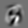
\includegraphics[width=.05\linewidth]{X_l_eigv_10.png}
    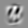
\includegraphics[width=.05\linewidth]{X_l_eigv_11.png}
    \caption{}
    \label{fig:modes_data}
  \end{subfigure}
  \begin{subfigure}{\linewidth}
    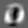
\includegraphics[width=.05\linewidth]{W_l_eigv_1.png}
    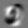
\includegraphics[width=.05\linewidth]{W_l_eigv_2.png}
    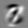
\includegraphics[width=.05\linewidth]{W_l_eigv_3.png}
    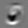
\includegraphics[width=.05\linewidth]{W_l_eigv_4.png}
    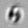
\includegraphics[width=.05\linewidth]{W_l_eigv_5.png}
    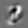
\includegraphics[width=.05\linewidth]{W_l_eigv_6.png}
    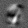
\includegraphics[width=.05\linewidth]{W_l_eigv_7.png}
    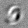
\includegraphics[width=.05\linewidth]{W_l_eigv_8.png}
    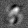
\includegraphics[width=.05\linewidth]{W_l_eigv_9.png}
    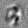
\includegraphics[width=.05\linewidth]{W_l_eigv_10.png}
    \caption{}
    \label{fig:modes_tr}
  \end{subfigure}\par
  \begin{subfigure}{\linewidth}
    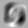
\includegraphics[width=.05\linewidth]{W_10_l_eigv_1.png}
    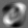
\includegraphics[width=.05\linewidth]{W_10_l_eigv_2.png}
    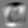
\includegraphics[width=.05\linewidth]{W_10_l_eigv_3.png}
    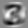
\includegraphics[width=.05\linewidth]{W_10_l_eigv_4.png}
    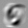
\includegraphics[width=.05\linewidth]{W_10_l_eigv_5.png}
    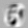
\includegraphics[width=.05\linewidth]{W_10_l_eigv_6.png}
    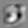
\includegraphics[width=.05\linewidth]{W_10_l_eigv_7.png}
    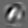
\includegraphics[width=.05\linewidth]{W_10_l_eigv_8.png}
    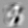
\includegraphics[width=.05\linewidth]{W_10_l_eigv_9.png}
    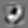
\includegraphics[width=.05\linewidth]{W_10_l_eigv_10.png}
    \caption{}
    \label{fig:modes_tr_10}
  \end{subfigure}
   \caption{\textbf{(a)} First mode learnt by the RBM with the external visible field initialized as a null vector. \textbf{(b)} External visible field initialized with rule \eqref{eq:bias_init}. \textbf{(c)} First principal components extracted from the training set. \textbf{(d)} Principal components extracted from the training set (starting from the second). \textbf{(e)} The first 10 modes of a trained RBM when rule \eqref{eq:bias_init}  has been used - 1 epoch.}
\end{figure}

The first 10 left singular vectors of a trained RBM are shown in fig. \ref{fig:modes_tr}. They are all composed by a homogeneous background on the borders and a set of alternating dark and light traits in the center, highlighting the fact that each singular vector acts globally on the visible layer. Even if the pictures seen in fig. \ref{fig:modes_tr} are quite different one from another, an interesting trend is found: a higher number of alternating traits is present in the successive vectors. At this point it is useful to draw a comparison to the Fourier decomposition of an image and interpret the left singular values as the \textit{modes} composing the activation pattern. The first singular vectors, characterized by a small number of alternating traits, play the role of the \textit{low frequency} modes while the successive modes act as \textit{high frequency} modes. The analogy to Fourier modes is suggested by the fact that we are basically performing Principal Component Analysis (PCA) over the matrix \textbf{W} and the left singular vectors can thus be identified with the principal modes of variation.

Looking at the dynamics of the learning it is seen that the modes take shape one by one as the corresponding singular value \(\sigma_j\) is brought above threshold. The subsequent strengthening of the \(\sigma_j\) corresponds to refinements and rotations, with little effects on the characterization of the modes as high or low frequency modes. For what concerns the modes below threshold, they present a dark border and a random configuration in the center; in this case the only effect of the training is to discern what are the units which are never activated and no information about the actual structure of the data is found.

These observations suggest that the RBM is able to learn the modes that compose the activation patterns of the data, starting with the low frequency modes and proceeding with the high frequency ones. Moreover, with reference to the \(\sigma_j\) distribution (fig. \ref{fig:sv4}), we note that the low frequency modes are given a higher weigth.

The dynamics described here and in the previous section present some similarities to the learning dynamics for deep linear neural networks \cite{ganguli}. Some insights on the behaviour of a RBM in the linear regime were given by looking at the SVD-like equations \eqref{eq:svd-like}, where we have seen how the magnetizations aligned to the strongest SVD modes are amplified. These magnetizations are thus unstable and they drive the formation of new mean-field fixed points during learning, that correspond to the magnetizations affine to the samples in the training set. These observations suggest a connection between the SVD of the data in the training set and the SVD of the weights matrix \(\mathbf{W}\), at least in the linear regime. This hypothesis is confirmed by comparing the SVD modes extracted from the data and those of the \(\mathbf{W}\) matrix, fig. \ref{fig:modes_lin}-\ref{eq:modes_data}, that are very similar. Going on with the training we expect non-linear effects to kick-in and this is seen in fig. \ref{fig:modes_tr} where the SVD of the data is not comparable to the SVD of \(\mathbf{W}\) anymore.

Summarizing, the analysis of the left singular vectors gives many insights on the training procedure:

\begin{itemize}
\item a RBM is able to learn the modes that compose the activation patterns of the training data
\item the low frequency modes are learnt first and are given higher weigths
\item at the beginning of the training the RBM operates in the linear regime and the \(\mathbf{W}\) matrix is shaped according to the SVD of the data in the training set
\item by continuing the training, new modes at increasing higher frequency are learnt while the already learnt modes are strengthen
\item the external visible field is equivalent to a left singular vector but we can avoid to learn it by using the appropriate initial conditions
\end{itemize}

Finally, the above observations suggest that the weights matrix of a trained RBM is composed by two classes of modes and we can express its components as

\begin{equation}
w_{i,j} = \sum_{\alpha \in bulk} \sigma_{\alpha} u_{i,\alpha} v_{j,\alpha} + \sum_{\alpha \in outliers} \sigma_{\alpha} u_{i,\alpha} v_{j,\alpha} 
\end{equation}

where \(u_{i,j}\) and \(v_{i,j}\) are the components of the \(\mathbf{U}\) and \(\mathbf{V}\) matrices of the SVD of \(\mathbf{W}\).

\section{Role of the modes}
By looking at the singular values distribution of \(\mathbf{W}\) we have seen that there seem to be \textit{more} and \textit{less important} singular vectors. In the previous section we have then refined this observation by highlighting how the lowest-frequency modes are given the highest weights. We can then identify the more (less) important modes as the low (high) frequency ones. To gain some intuition about the meaning of this separation we can take our analogy further and think about the Fourier decomposition of a square wave; in such a case, the superposition of the low frequency harmonics is sufficient to build a good approximation of a square wave, while the role of the high frequency harmonics is that of sharpening the waveform at the discontinuity points. In the context of a trained RBM, we then expect that good approximations to the training data are obtained by exploiting only the low frequency modes, while the high frequency modes should represent minor corrections.

\begin{figure}
  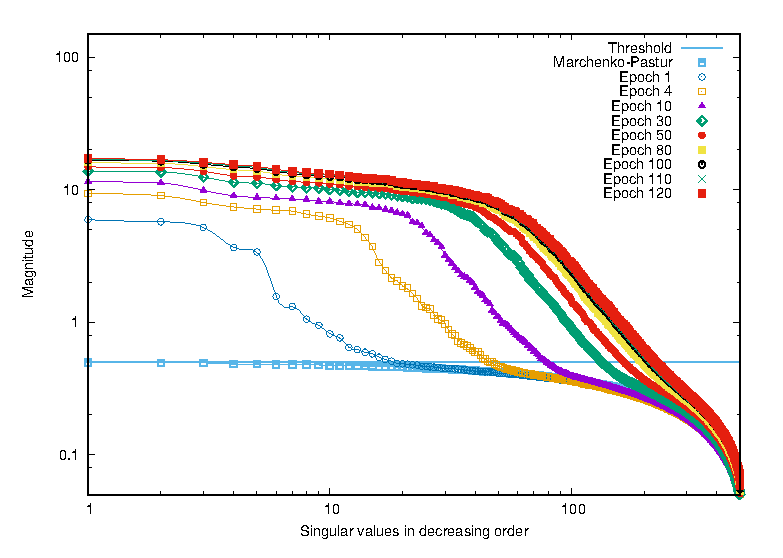
\includegraphics{SV_pl.eps}
  \caption{Singular values}
  \label{fig:sv_pl}
\end{figure}

It is not clear, however, how we can discern between high and low frequency modes. Some hints to address this issue are given by looking at the value of the \(\sigma_j\) in decreasing order on a log-log plot (fig. \ref{fig:sv_pl}), in which an interesting picture emerges: the strongest \(\sigma_j\) are located far above threshold and are of comparable magnitude, followed by a tail of exponentially damped \(\sigma_j\). This picture is consistent across the training, the only difference being the damping cutoff that is increasing with the epochs. After a long training, however, the increase in the cutoff is very slow and this could serve as a signal to stop the learning, as such situation amounts to slowly strengthening singular values which are exponentially less important then the already learnt modes.

We are then driven to define the more important low frequency modes as the modes before cutoff, and the exponentially less important high frequency modes as those after cutoff. A consistency check is shown in fig. \ref{fig:hf_modes}, where just the 100 strongest modes are retained to construct the samples and the remaining modes are shown to encode boundary corrections. Choosing the first 100 modes is arbitrary; in fig. \ref{fig:sv_pl} we can see how the cutoff is well below 100, so with this choice we are sure that we included in the reconstruction of the samples all the strong modes before cutoff plus a small number of modes giving boundary corrections.

\begin{figure}
  \begin{subfigure}{\linewidth}
  	\centering
    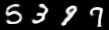
\includegraphics[width=.4\linewidth]{complete40ep.png}
    \caption{}
  \end{subfigure}\par
  \begin{subfigure}{\linewidth}
  	\centering
    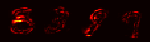
\includegraphics[width=.4\linewidth]{difference20ep.png}
    \caption{}  
  \end{subfigure}\par
  \begin{subfigure}{\linewidth}
  	\centering
    \includegraphics[width=.4\linewidth]{difference40ep.png}
    \caption{}
  \end{subfigure}
  \caption{\textbf{(a)} The image shows some samples obtained with the trained RBM (after a 40 epochs training) and then "filtered" by eliminating the 400 weakest modes (just the 100 strongest modes are retained). \textbf{(b)} The images are composed by eliminating the 100 strongest modes to see what the weakest modes actually encode (20 epochs training). \textbf{(c)} As in \textbf{(b)} but after a 40 epochs training.}
  \label{fig:hf_modes}
\end{figure}

 
\begin{thebibliography}{9}

\bibitem{go}
D. Silver et al., "Mastering the game of Go with deep neural networks and tree search",
\textit{Nature}, 529, p. 484–489, 2016.

\bibitem{foundations}
F. Cucker, S. Smale, "On the mathematical foundations of learning",
\textit{Bull. Amer. Math. Soc.}, 39, p. 1-49, 2002.

\bibitem{hist1}
W. Krauth, M. Mezard, "Machine Learning algorithms with optimal stability in neural networks",
\textit{Journal of Physics A: Mathematical and General}, 20, L745–L752, 1987.

\bibitem{hist2}
J. J. Hopfield, "Neural networks and physical systems with emergent collective computational abilities"\textit{Proceedings of the National Academy of Sciences, 79}, 8, p. 2554–2558, 1982.

\bibitem{tap_train}
M. Gabri\'e, E. W. Tramel, F. Krzakala,
Training Restricted Boltzmann Machines via the Thouless-Anderson-Palmer Free Energy,
\textit{Advances in Neural Information Processing Systems (NIPS)}, 28, pages 640--648, 2015.

\bibitem{tap}
E. W. Tramel, M. Gabri\'e, A. Manoel, F. Caltagirone, F. Krzakala, \textit{arXiv:1702.03260}

\bibitem{monasson}
J. Tubiana, R. Monasson, "Emergence of Compositional Representations in Restricted Boltzmann Machines",
\textit{Phys. Rev. Lett. 118, 138301}, 2017.

\bibitem{Hinton_CD}
G. E. Hinton, “Training products of experts by minimizing Contrastive divergence,”
\textit{Neural computation}
, vol. 14, pp. 1771-1800, 2002.

\bibitem{PCD}
T. Tieleman, “Training restricted Boltzmann machines using approximations to the likelihood gradient,”
\textit{ICML}, Vol. 307, p. 7, 2008.

\bibitem{Hinton_guide}
G. E. Hinton, "A Practical Guide to Training Restricted Boltzmann Machines", \textit{Proceedings of Neural Networks: Tricks of the Trade (2nd ed.)}, pages 599-619, 2012. 

\bibitem{PCA}
I.T. Jolliffe, "Principal Component Analysis",
\textit{Springer-Verlag New York}, 2002.

\bibitem{SK}
D. Sherrington, S. Kirkpatrick,
"Solvable Model of a Spin-Glass",
\textit{Phys. Rev. Lett.}, Vol. 35, 1975.

\bibitem{ht_exp}
A. Georges, J. S. Yedidia,
"How to expand around mean-field theory using high-temperature expansions",
\textit{Journal of Physics A: Mathematical and General}, Volume 24, Number 9, 1991

\bibitem{TAP}
D. J. Thouless , P. W. Anderson, R. G. Palmer,
"Solution of 'Solvable model of a spin glass'",
\textit{Philosophical Magazine}, Vol. 35:3, p. 593-601, 1977

\bibitem{conv}
E. Bolthausen, "An Iterative Construction of Solutions of the TAP Equations for the Sherrington–Kirkpatrick Model", \textit{Commun. Math. Phys.}, Vol. 325, pages 333-366, 2014.

\bibitem{mnist}
http://yann.lecun.com/exdb/mnist/

\bibitem{gibbs}
G. Casella and E. I. George, "Explaining the Gibbs Sampler",
\textit{The American Statistician},
Vol. 46, No. 3, pp. 167-174, 1992.

\bibitem{leroy}
C. Leroy made an investigation on TAP fixed points and free energy landscape while at Laboratoire de Recherche en Informatique, working in my same team.

\bibitem{Nishimori}
H. Nishimori, "Statistical Physics of Spin Glasses and Information Processing: An Introduction",
\textit{Oxford University Press}, 2001

\bibitem{MP_law}
Marchenko, V.A. and Pastur, L.A., "Distribution of Eigenvalues for Some Sets of Random Matrices", \textit{Sbornik: Mathematics}, Vol. 1, pages 457-483, 1967.

\bibitem{ganguli}
A. M. Saxe, J. L. McClelland, S. Ganguli, "Exact solutions to the nonlinear dynamics of learning in deep linear neural networks",
\textit{arXiv:1312.6120}, 2014.

\end{thebibliography}


\end{document}
